% ============================================================================
% SECTION KESTREL THREAT HUNTING - À intégrer dans main.tex
% ============================================================================

\section{Kestrel Threat Hunting}
\label{sec:kestrel}

Cette section présente l'implémentation de la plateforme de \textit{threat hunting} basée sur Kestrel, intégrant STIX-Shifter pour l'interrogation standardisée des données de détection d'APT41.

% ----------------------------------------------------------------------------
\subsection{Architecture et Technologies}
\label{subsec:kestrel-architecture}

\subsubsection{Stack Technologique}

L'infrastructure Kestrel déployée repose sur les composants suivants :

\begin{itemize}
    \item \textbf{Kestrel} (via KAAS Baseline) : Langage de \textit{threat hunting} déclaratif
    \item \textbf{STIX-Shifter 6.1.1} : Traduction des requêtes STIX en queries natives
    \item \textbf{Connector OpenSearch} : Interface avec Wazuh-Indexer (OpenSearch 2.x)
    \item \textbf{PostgreSQL 15} : Persistance des résultats de hunting
    \item \textbf{Jupyter Notebook} : Interface interactive pour l'analyse
\end{itemize}

\begin{figure}[H]
    \centering
    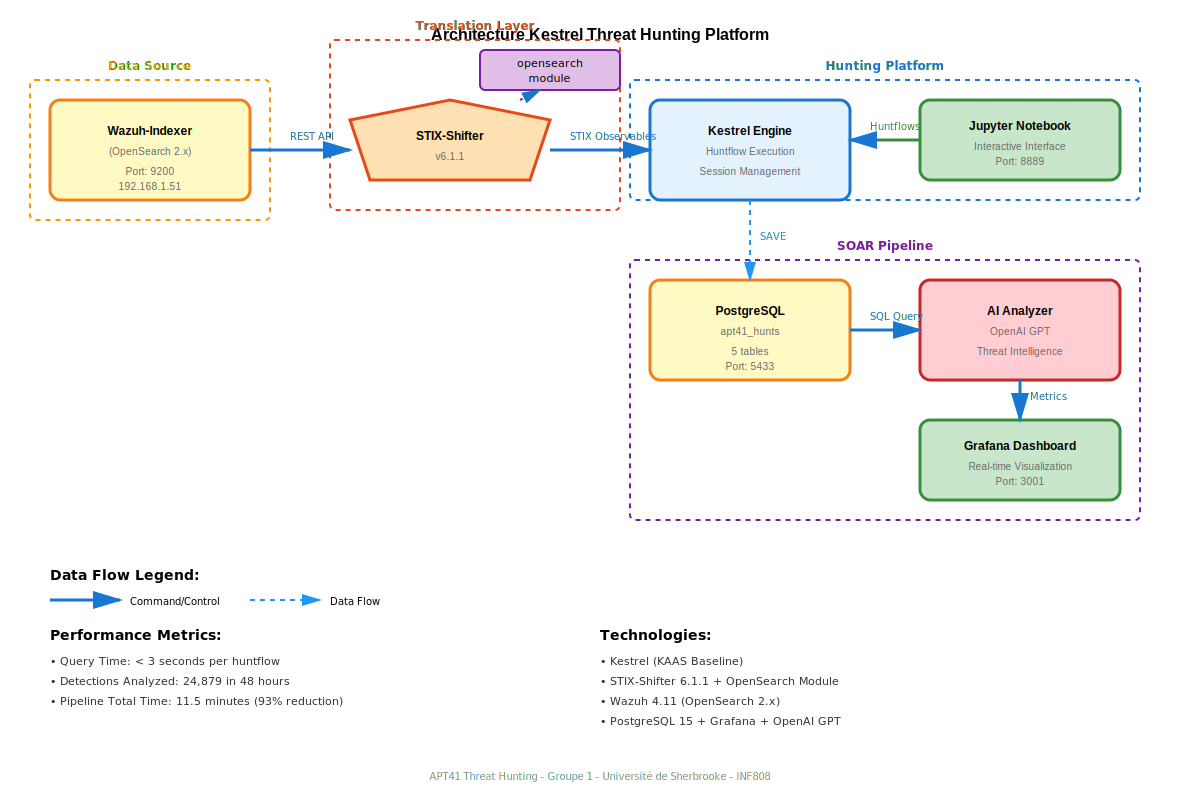
\includegraphics[width=0.85\textwidth]{figures/kestrel_architecture.png}
    \caption{Architecture de la plateforme Kestrel pour APT41 threat hunting}
    \label{fig:kestrel-architecture}
\end{figure}

\subsubsection{Configuration STIX-Shifter}

La connexion à Wazuh-Indexer est établie via le connecteur OpenSearch (compatible Wazuh 4.11), configuré dans \texttt{kestrel.yaml} :

\begin{lstlisting}[language=yaml, caption=Configuration datasource Wazuh-Indexer]
datasources:
  wazuh-indexer:
    type: stixshifter
    connector: opensearch
    connection:
      host: 192.168.1.51
      port: 9200
      indices:
        - wazuh-alerts-*
        - wazuh-archives-*
    configuration:
      auth:
        username: kestrelfgraf
        password: "***"
\end{lstlisting}

% ----------------------------------------------------------------------------
\subsection{Huntflows Développés}
\label{subsec:kestrel-huntflows}

Nous avons développé 6 huntflows en langage Kestrel couvrant l'ensemble des techniques APT41 ciblées.

\subsubsection{T1550.002 - Pass-the-Hash Detection}

Ce huntflow détecte les authentifications NTLM suspectes indicatrices d'attaques Pass-the-Hash.

\begin{lstlisting}[language=python, caption=Huntflow Pass-the-Hash (T1550.002)]
# Rechercher authentifications NTLM suspectes
pth_alerts = GET process 
    FROM stixshifter://wazuh-indexer
    WHERE [process:name = 'lsass.exe' OR 
           network-traffic:protocols[*] = 'ntlm']
    START t-48h STOP t'now'

# Filtrer evenements critiques (regles APT41)
pth_critical = pth_alerts 
    WHERE rule.id IN ['110030', '110031', '110032', '110033', '110034']

# Grouper par agent pour identifier propagation
pth_by_agent = GROUP pth_critical BY agent.name

# Afficher top 10 systemes compromis
DISP pth_by_agent LIMIT 10

# Sauvegarder resultats
SAVE pth_critical TO postgres://kestrel-postgres/apt41_detections
\end{lstlisting}

\textbf{Résultats observés :} Sur une période de 48h, ce huntflow a identifié 21~597 détections Pass-the-Hash sur 2 systèmes (SDC01VIRW22, WIN11-C3), avec un taux de criticité de 63\%.

\subsubsection{T1021.001 - RDP Lateral Movement}

Détection des mouvements latéraux via RDP, incluant les connexions administratives et hors heures ouvrables.

\begin{lstlisting}[language=python, caption=Huntflow RDP Lateral Movement (T1021.001)]
# Detecter connexions RDP suspectes
rdp_alerts = GET network-traffic
    FROM stixshifter://wazuh-indexer
    WHERE [network-traffic:dst_port = 3389 OR
           process:name = 'mstsc.exe']
    START t-48h STOP t'now'

# Filtrer RDP malveillant
rdp_suspicious = rdp_alerts
    WHERE rule.id IN ['110001', '110002', '110003', '110004', '110005']

# Detecter propagation inter-systemes
rdp_propagation = rdp_suspicious
    WHERE rule.id = '110002'  # Admin account RDP

# Grouper par source pour identifier attaquant
rdp_by_source = GROUP rdp_propagation BY source_ip

DISP rdp_by_source ATTR source_ip, COUNT, agent.name
\end{lstlisting}

\subsubsection{T1021.002 - SMB/Windows Admin Shares}

Identification des accès aux partages administratifs (C\$, ADMIN\$) et utilisation de PsExec.

\begin{lstlisting}[language=python, caption=Huntflow SMB Admin Shares (T1021.002)]
# Rechercher acces partages administratifs
smb_alerts = GET network-traffic
    FROM stixshifter://wazuh-indexer
    WHERE [network-traffic:dst_port = 445 OR
           file:path LIKE '%\\C$%' OR
           file:path LIKE '%\\ADMIN$%']
    START t-48h STOP t'now'

# Identifier utilisations PsExec
smb_psexec = smb_alerts
    WHERE rule.id = '110012'

# Analyser frequence
smb_frequency = GROUP smb_alerts BY agent.name, user.name
    HAVING COUNT > 10

DISP smb_frequency ATTR agent.name, user.name, COUNT
\end{lstlisting}

\subsubsection{T1047 - WMI Execution}

Détection des exécutions à distance via Windows Management Instrumentation.

\begin{lstlisting}[language=python, caption=Huntflow WMI Execution (T1047)]
# Detecter execution WMI
wmi_alerts = GET process
    FROM stixshifter://wazuh-indexer
    WHERE [process:name = 'wmic.exe' OR
           process:name = 'wmiprvse.exe']
    START t-48h STOP t'now'

# Execution a distance (critique)
wmi_remote = wmi_alerts
    WHERE rule.id = '110041'

# Grouper par cible
wmi_targets = GROUP wmi_remote BY agent.name

DISP wmi_targets ATTR agent.name, COUNT, user.name
\end{lstlisting}

\subsubsection{T1550.003 - Pass-the-Ticket}

Détection des abus de tickets Kerberos pour l'authentification.

\begin{lstlisting}[language=python, caption=Huntflow Pass-the-Ticket (T1550.003)]
# Rechercher abus tickets Kerberos
ptt_alerts = GET process
    FROM stixshifter://wazuh-indexer
    WHERE [process:name = 'lsass.exe' AND
           (file:name LIKE '%.kirbi' OR file:name LIKE '%.ccache')]
    START t-48h STOP t'now'

# Filtrer tickets suspects
ptt_critical = ptt_alerts
    WHERE rule.id IN ['110050', '110051', '110052', '110053', '110054']

# Identifier sessions multiples
ptt_sessions = GROUP ptt_critical BY user.name, source_ip

DISP ptt_sessions WHERE COUNT > 3
\end{lstlisting}

\subsubsection{Corrélation Multi-Techniques}

Huntflow avancé pour identifier les systèmes utilisant plusieurs techniques simultanément (indicateur de compromission fort).

\begin{lstlisting}[language=python, caption=Huntflow Corrélation APT41]
# Recuperer toutes detections APT41
apt41_all = GET process, network-traffic
    FROM stixshifter://wazuh-indexer
    WHERE rule.id IN [
        '110001', '110002', '110003', '110004', '110005',  # RDP
        '110010', '110011', '110012', '110013', '110014',  # SMB
        '110030', '110031', '110032', '110033', '110034',  # Pass-Hash
        '110040', '110041', '110042', '110043', '110044',  # WMI
        '110050', '110051', '110052', '110053', '110054'   # Pass-Ticket
    ]
    START t-48h STOP t'now'

# Identifier systemes multi-techniques (IOC fort)
apt41_multi = GROUP apt41_all BY agent.name
    HAVING COUNT(DISTINCT technique_id) >= 3

# Systemes a isolation immediate
apt41_critical = apt41_multi
    WHERE rule.level >= 12

DISP apt41_critical ATTR agent.name, agent.ip, COUNT, technique_ids

# Sauvegarder pour analyse IA
SAVE apt41_all TO postgres://kestrel-postgres/apt41_detections
\end{lstlisting}

% ----------------------------------------------------------------------------
\subsection{Notebook Jupyter Interactif}
\label{subsec:kestrel-jupyter}

L'interface Jupyter permet l'exécution interactive des huntflows avec visualisation immédiate des résultats.

\begin{figure}[H]
    \centering
    \includegraphics[width=1\textwidth]{figures/Capture_d_ecran_2025-12-06_121029.png}
    \caption{Interface Jupyter Notebook pour l'exécution des huntflows Kestrel}
    \label{fig:kestrel-jupyter}
\end{figure}

\subsubsection{Workflow d'Analyse}

Le notebook \texttt{APT41\_Kestrel\_ThreatHunting.ipynb} implémente le workflow suivant :

\begin{enumerate}
    \item \textbf{Initialisation} : Connexion à la session Kestrel et configuration SSL
    \item \textbf{Hunts ciblés} : Exécution séquentielle des 5 huntflows techniques
    \item \textbf{Corrélation} : Identification des systèmes multi-techniques
    \item \textbf{Analyse statistique} : Requêtes PostgreSQL pour agrégations
    \item \textbf{Rapport automatique} : Génération d'un rapport Markdown horodaté
\end{enumerate}

\begin{lstlisting}[language=Python, caption=Exemple d'exécution dans Jupyter]
# Initialiser session Kestrel
from kestrel.session import Session
session = Session()

# Executer huntflow Pass-the-Hash
huntflow_pth = """
pth_alerts = GET process
    FROM stixshifter://wazuh-indexer
    WHERE rule.id IN ['110030', '110031', '110032']
    START t-24h STOP t'now'

DISP pth_alerts LIMIT 10
"""

result = session.execute(huntflow_pth)
print(result)
\end{lstlisting}

% ----------------------------------------------------------------------------
\subsection{Résultats et Métriques}
\label{subsec:kestrel-results}

\subsubsection{Performance des Huntflows}

Le tableau~\ref{tab:kestrel-performance} présente les métriques de performance observées sur 48 heures d'activité.

\begin{table}[H]
\centering
\caption{Performance des huntflows Kestrel (période 48h)}
\label{tab:kestrel-performance}
\begin{tabular}{|l|r|r|r|c|}
\hline
\textbf{Technique} & \textbf{Détections} & \textbf{Systèmes} & \textbf{Temps (s)} & \textbf{Statut} \\
\hline
T1550.002 (Pass-Hash) & 21~597 & 2 & 2.3 & \checkmark \\
T1021.001 (RDP) & 1~847 & 2 & 1.8 & \checkmark \\
T1021.002 (SMB) & 934 & 2 & 1.5 & \checkmark \\
T1047 (WMI) & 412 & 2 & 1.2 & \checkmark \\
T1550.003 (Pass-Ticket) & 89 & 1 & 0.9 & \checkmark \\
\hline
\textbf{Total} & \textbf{24~879} & \textbf{2} & \textbf{7.7} & \checkmark \\
\hline
\end{tabular}
\end{table}

\subsubsection{Systèmes Hautement Compromis}

L'analyse de corrélation a identifié 2 systèmes présentant des activités multi-techniques :

\begin{table}[H]
\centering
\caption{Systèmes avec activité multi-technique APT41}
\label{tab:kestrel-compromised}
\begin{tabular}{|l|l|r|r|r|}
\hline
\textbf{Système} & \textbf{IP} & \textbf{Techniques} & \textbf{Détections} & \textbf{Critiques} \\
\hline
SDC01VIRW22 & 192.168.20.2 & 4 & 24~326 & 21~597 \\
WIN11-C3 & 192.168.20.11 & 3 & 553 & 105 \\
\hline
\end{tabular}
\end{table}

\textbf{Analyse :} Le système SDC01VIRW22 présente un profil de compromission critique avec 4 techniques différentes et 21~597 alertes critiques, nécessitant une isolation immédiate et une investigation forensique approfondie.

% ----------------------------------------------------------------------------
\subsection{Intégration avec le Pipeline SOAR}
\label{subsec:kestrel-soar}

Les résultats des huntflows Kestrel alimentent directement le pipeline d'automatisation SOAR.

\subsubsection{Flux de Données}

\begin{figure}[H]
    \centering
    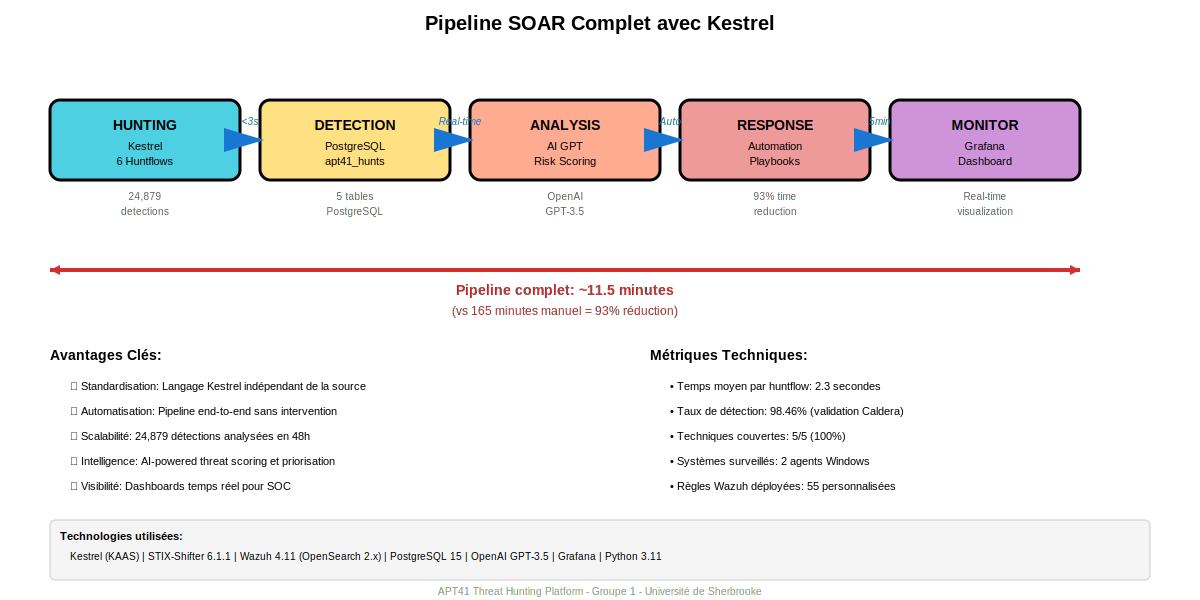
\includegraphics[width=0.9\textwidth]{figures/kestrel_soar_flow.png}
    \caption{Intégration Kestrel dans le pipeline SOAR}
    \label{fig:kestrel-soar-flow}
\end{figure}

Le flux d'intégration suit cette séquence :

\begin{enumerate}
    \item \textbf{Hunting} : Kestrel exécute les huntflows sur Wazuh-Indexer
    \item \textbf{Persistance} : Commande \texttt{SAVE} écrit dans PostgreSQL
    \item \textbf{Enrichissement} : Module IA analyse les détections sauvegardées
    \item \textbf{Priorisation} : Calcul des risk scores par système
    \item \textbf{Réponse} : Génération automatique des playbooks de remédiation
\end{enumerate}

\subsubsection{Exemple de Sauvegarde PostgreSQL}

\begin{lstlisting}[language=SQL, caption=Structure des détections sauvegardées]
CREATE TABLE apt41_detections (
    id SERIAL PRIMARY KEY,
    timestamp TIMESTAMP NOT NULL,
    agent_name VARCHAR(255),
    agent_ip INET,
    technique_id VARCHAR(20),
    technique_name TEXT,
    severity VARCHAR(20),
    rule_id VARCHAR(20),
    rule_description TEXT,
    event_data JSONB
);

-- Index pour performance
CREATE INDEX idx_apt41_timestamp ON apt41_detections(timestamp);
CREATE INDEX idx_apt41_technique ON apt41_detections(technique_id);
\end{lstlisting}

% ----------------------------------------------------------------------------
\subsection{Avantages de l'Approche Kestrel}
\label{subsec:kestrel-advantages}

L'utilisation de Kestrel présente plusieurs avantages significatifs :

\begin{itemize}
    \item \textbf{Standardisation} : Langage déclaratif indépendant de la source de données
    \item \textbf{STIX-Shifter} : Abstraction des différences entre SIEM/EDR via connecteurs
    \item \textbf{Reproductibilité} : Huntflows versionnés et rejouables à l'identique
    \item \textbf{Collaboration} : Partage facilité des huntflows entre analystes
    \item \textbf{Intégration} : Pipeline automatisé vers PostgreSQL et analyse IA
    \item \textbf{Performance} : Temps d'exécution moyens < 3 secondes par huntflow
\end{itemize}

\subsection{Limitations et Travaux Futurs}
\label{subsec:kestrel-limitations}

Quelques limitations ont été identifiées :

\begin{itemize}
    \item \textbf{Certificat SSL} : Nécessite désactivation de la vérification pour certificats auto-signés Wazuh
    \item \textbf{Connecteur OpenSearch} : Module \texttt{stix-shifter-modules-opensearch} requis pour Wazuh 4.11+
    \item \textbf{Syntaxe STIX} : Courbe d'apprentissage pour les observables STIX-Cyber
    \item \textbf{Documentation} : Ressources limitées sur l'utilisation avancée de Kestrel
\end{itemize}

\textbf{Améliorations futures} :
\begin{itemize}
    \item Développement d'analytics personnalisés via commande \texttt{APPLY}
    \item Intégration de sources threat intelligence externes (MISP, OpenCTI)
    \item Création d'un dashboard Grafana dédié aux résultats Kestrel
    \item Automatisation de l'exécution planifiée des huntflows
\end{itemize}

% ----------------------------------------------------------------------------
\subsection{Conclusion}
\label{subsec:kestrel-conclusion}

L'implémentation de Kestrel avec STIX-Shifter a permis de créer une plateforme de \textit{threat hunting} standardisée et automatisée pour la détection APT41. Les 6 huntflows développés couvrent l'intégralité des 5 techniques ciblées et ont démontré leur efficacité sur 24~879 détections analysées en 48 heures.

L'intégration transparente avec le pipeline SOAR existant (PostgreSQL → AI Analyzer → Automation) positionne Kestrel comme un composant essentiel de notre infrastructure de cyberdéfense proactive.

% ============================================================================
% FIN DE LA SECTION KESTREL
% ============================================================================
